As it was mentionned in sec. \ref{sec:QSH}, the QSH effect requiers strong spin-orbit coupling to occur. Kane and Mele initially proposed that the effect could be realised in graphene but the spin-orbit coupling of carbon is too weak \cite{cayssol_topological_2021}. The first observed topological insulator with QSH effect is a mercury telluride heterostructure consisting of a staking of thin \ch{HgTe} layers between \ch{Hg_xCd_{1-x}Te} \cite{kane_this_2011}. The Band structure of \ch{HgTe} and \ch{Hg_xCd_{1-x}Te} both contain a $\Gamma_6$ and $\Gamma_8$ band \cite{bernevig_topological_2013}. While the $\Gamma_6$ band is $s$-type, the $\Gamma_8$ band is $p$-type. A $s$-type (resp. $p$-type) is formed with the hybridization of $s$ (resp. $p$) orbitals with $0$ (resp. $1$) angular momentum quantum number \cite{girvin_modern_2019}. Adding spin leads to $1/2$ and $3/2$ respective total angular momentum quantum number for $\Gamma_6$ and $\Gamma_8$ bands \cite{bernevig_topological_2013}. In \ch{HgTe}, the strong spin-orbit coupling leads the $\Gamma_8$ band to be more energetic than the $\Gamma_6$ band and the opposite is true for \ch{Hg_xCd_{1-x}Te} \cite{buhmann_quantum_2011}. A schematic view of the resulting quantum well structure is presented on fig. \ref{hg}.
\begin{figure}[h!]
    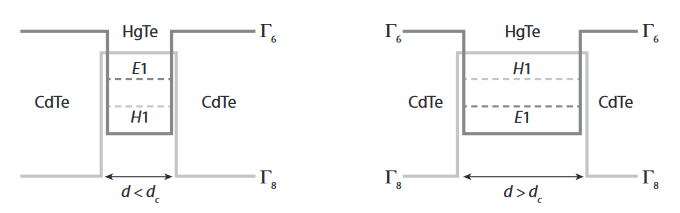
\includegraphics[scale=0.8]{sections/visuel/Hg}
    \caption{Schematic representation of the energies of the $\Gamma_6$ and $\Gamma_8$ bands in the \ch{HgTe}/\ch{Hg_xCd_{1-x}Te} quantum well structure \cite{bernevig_topological_2013}. The  $E1$ well level is the highest confined energy level from $\Gamma_6$ and the $H1$ level is the lowest confined level from $\Gamma_8$. $d$ is the thickness of the well and $d_c$ is the critical value for which $E1$ and $H1$ are reversed.}
    \label{hg}
\end{figure}
The most important feature of this structure for the realisation of the QSH effect is the fact it the levels $E1$ and $H1$ get inverted for sufficient well thickness $d$ (greater than the critical thickness $d_c$). Band inversion is the signature of the appearence of a topologial phase with variation of the thickness \cite{bansil_colloquium_2016}. Near the edges of the sample, translationnal symmetry breaks and the spin-orbit coupling loses intensity so that the $E1$ and $H1$ levels are inverted back. Gapless edge states emerge from this inversion (see fig. \ref{cross}) and they precisely correspond to the helical Kramer pair states mentionned in sec. \ref{sec:QSH} \cite{buhmann_quantum_2011}.  

\begin{figure}[h!]
    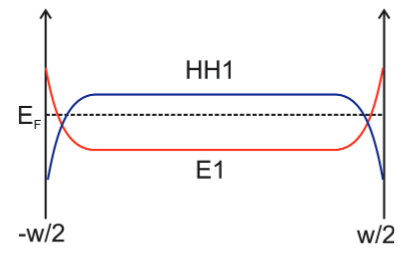
\includegraphics[scale=0.8]{sections/visuel/cross}
    \caption{Reinversion of the $E1$ and $H1$ levels near the edge of the sample of width $w$.}
    \label{cross}
\end{figure}